\documentclass[12pt,letterpaper]{article}
\usepackage[margin=0.6in]{geometry}
\usepackage[T1]{fontenc}
\usepackage{mathptmx}
\usepackage{graphicx}
\usepackage{microtype}
\usepackage[unicode,hidelinks]{hyperref}
\hypersetup{pdftitle={Rule context constrains the interchangeability of content-matched memory states},
  pdfauthor={},pdfsubject={Anonymous COSYNE submission},pdfcreator={LaTeX},pdfkeywords={}}
\pagestyle{empty}
\setlength{\parindent}{0pt}
\setlength{\parskip}{5pt}
\setlength{\emergencystretch}{1em}
% Slightly above the nominal requirements also in PDF (1 pt = 1/72 inch).
\AtBeginDocument{\fontsize{12.1}{14.35}\selectfont}
\newcommand{\blocktitle}[1]{\par\vspace{4pt}{\bfseries #1}\par\vspace{1pt}}
\begin{document}
\begin{center}
{\fontsize{16.1}{18}\selectfont\bfseries
Rule context constrains the interchangeability\\
of content-matched memory states}
\end{center}
\vspace{-5pt}
\blocktitle{Summary}
Working memory retains information for use under task rules. If memory states have the same content and similar representations, can we use them interchangeably in subsequent computation? Six independently initialized recurrent networks were trained on a permutation-based memory task. Each network received a permutation of 1 through 7, processed operation cues separated by delays, and answered queries about the resulting permutation. The operations included inversion and complementation (replacing each position label j with $8-j$). A preceding context cue determined whether A meant inversion and B complementation, or vice versa. Exact permutation relations allowed different initial inputs and histories to reach identical current permutations. Within each network, we replaced the memory component of the receiver's hidden state with the donor's while retaining the receiver's control component, subsequent inputs, and readout. Exchanges within the same rule context introduced new errors on 1.7\% of all queries, compared with 53.4\% across contexts. Under identical subsequent inputs, answers after exchange matched the donor's own answers on $>99.99$\% of queries, including nearly all donor errors. Some paired control states were identical. Translating subsequent cues into their donor-context equivalents increased cross-context accuracy from 42.1\% to 97.9\% on held-out permutations; the same translation without exchange reduced original-task accuracy from 97.9\% to 42.1\%. Linear centered kernel alignment (CKA) distributions largely overlapped between within-context and cross-context pairs (medians approximately 0.892 and 0.889). Adding CKA to a baseline accounting for task conditions, native performance, content decoding, and input/control-state distances did not consistently improve loss predictions for held-out networks and condition pairs. These results suggest that content-matched memory states can carry different information about how subsequent cues are interpreted. In these networks, matching content and high CKA did not guarantee functional interchangeability, motivating causal tests when interpreting neural population representations.


\blocktitle{Additional Detail}
The intervention uses two trials in the same trained network (Fig.~1A).
Their initial permutations and cue histories can differ while producing exactly
the same current permutation. The architecture partitions the hidden state into
memory $m$ and control $c$. We replace $m_R$ with $m_D$ in native coordinates,
then use the receiver's subsequent inputs and the unchanged network readout.
Retaining $c_R$ specifies a component intervention; it does not establish that
the receiver's functional rule is retained. Some paired control states are
exactly equal. Intervention definitions and scoring matter for interpretation [2].

New errors count native-correct, exchange-wrong answers divided by \emph{all}
evaluated queries (Fig.~1B; 134 B1 permutations, 19 orbits). Means weight networks
equally; within each network, condition pairs, both directions, delays
$d=0,10$, and suffixes NN/NA/NB retain their original weights. Each permutation
has seven item-to-position and seven position-to-item queries. Cue translation
swaps A/B and preserves N. Both treatments in Fig.~1C are scored against the
\emph{original} receiver target, including NN. The no-exchange control is native,
unpatched activity. Its 362 B\_reserved permutations (51 orbits) were held out
from earlier B1 exploration; this submission reuses saved results.

Linear CKA [1] uses content-aligned memory states from the separate geometry set
G. Figure~1D uses only $d=0$, with each network--unordered-condition pair counted
once across suffixes. Its pooled median is not the mean of network medians.
The original held-out-network/unseen-pair predictor comparison gave mean MAE
improvement $-0.0149$ nat with CKA (one of six folds positive); the original
refit-bootstrap 95\% interval was very wide, $[-42.56,87.78]$ nat. This limits
precision and does not show that CKA is generally uninformative.
Network 106 and weak native conditions remain included.
Registered GPU checks passed; the original strict CPU float32 logit tolerance
failed (float64 agreed; compared argmax answers were unchanged).
These findings concern the tested networks and continuations.

\newpage
\noindent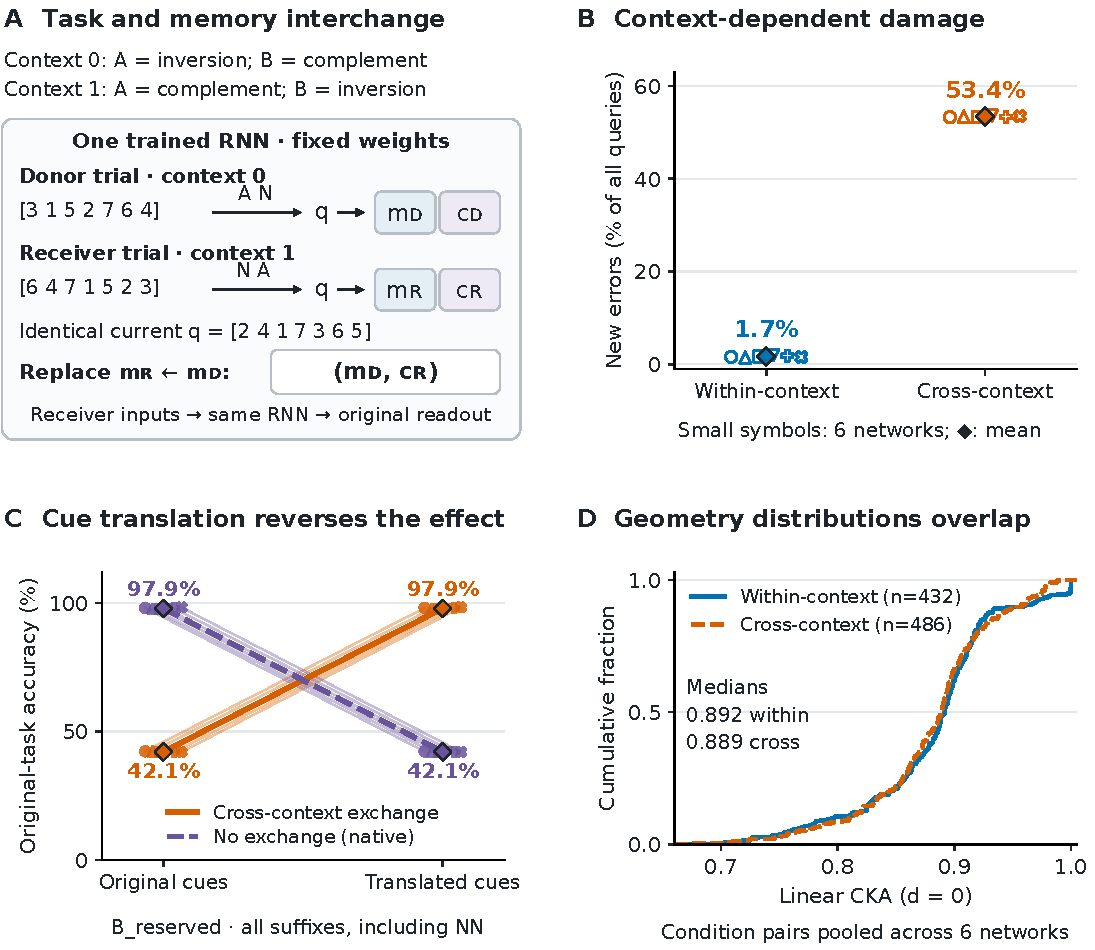
\includegraphics[width=\linewidth]{figures/figure_1.pdf}\par
\vspace{-3pt}
{\fontsize{10.1}{11.9}\selectfont
\textbf{Figure 1. Rule context changes the functional use of matched memory.}
\textbf{A,} Two trials in one fixed network reach the same full permutation
$q$ from different initial inputs and histories (N is a no-operation cue).
The exchanged state is $(m_D,c_R)$; keeping $c_R$ does not imply retaining the
receiver's functional rule, and $c_D$ need not differ from $c_R$.
\textbf{B,} New-error percentages use all B1 queries as denominator; small
symbols show six independently trained networks (seeds 101--106), and diamonds
show their equal-weight means.
\textbf{C,} On B\_reserved, translating cues compensates cross-context exchange
but impairs native, unexchanged performance on the original target. Thin paired
lines/small symbols show networks; thick lines/diamonds show equal-weight means.
Seed symbols in B/C follow the same order: circle, up-triangle, square,
down-triangle, filled plus, X; horizontal offsets separate overlapping marks.
All prespecified suffixes, including NN, and both delays contribute to B/C.
\textbf{D,} ECDFs pool 432 within-context and 486 cross-context geometric
measurements at $d=0$ (72/81 unordered condition pairs per network), with no
suffix duplication. These are dependent condition-level distributions across
six networks, not 918 independent training runs. Blue/orange denote
within/cross context in B/D. Identical future inputs gave $>99.99\%$
donor-answer agreement, including nearly all donor errors.
\par}
\vspace{2pt}
{\fontsize{10.1}{11.8}\selectfont
\textbf{References}\par
\vspace{-2pt}
[1] Kornblith, S., Norouzi, M., Lee, H. \& Hinton, G. (2019).
Similarity of Neural Network Representations Revisited.
\emph{PMLR} 97, 3519--3529.
\href{https://proceedings.mlr.press/v97/kornblith19a.html}{proceedings.mlr.press/v97/kornblith19a.html}\par
\vspace{-2pt}
[2] Zhang, F. \& Nanda, N. (2024).
Towards Best Practices of Activation Patching in Language Models: Metrics and Methods.
\emph{ICLR}. \href{https://arxiv.org/abs/2309.16042}{arXiv:2309.16042}.
\par}
\end{document}
